\documentclass{beamer}

\mode<presentation>{
\usetheme{CambridgeUS}
}

\setbeamertemplate{footline}[page number]

\usepackage[utf8]{inputenc}
\usepackage[ngerman]{babel}
\usepackage{graphicx}
\usepackage{multirow}
\usepackage{adjustbox}
\usepackage{array}
\usepackage{colortbl}	

\usepackage{xcolor}
\usepackage{tikz} %Zeichnungen

\definecolor{darkblue}{rgb}{0, 0, 0.4}
\definecolor{cornellred}{rgb}{0.7, 0.11, 0.11}

\title[Elektrizitätslehre]{LCR-Schwingkreis und gekoppelte LC-Schwingkreise}
\author{Simon Schwarz}
\institute{Grundpraktikum Physik Teil I}
\date{25. September 2019}


\begin{document}

%Titelseite
\begin{frame}
\titlepage
\end{frame}

%Inhaltsverzeichnis
\begin{frame}
\frametitle{Inhalt}
\tableofcontents
\end{frame}


\section{LCR-Schwingkreis}
\subsection{Theorie}

\begin{frame}
\centering
\Large{LCR-Schwingkreis}
\end{frame}

\begin{frame}
\frametitle{Die Differentialgleichung des LCR-Schwingkreises}

\begin{columns}[c]
\column{.7\textwidth}

Kirchhoffsche Maschenregel: $U_0 = U_R + U_L + U_C = R\cdot I + L\frac{dI}{dt} + \frac{Q}{C}$ \\
Mit $I = \frac{dQ}{dt}$ folgt:
\begin{block}{Differentialgleichung (Gedämpfte Schwingung)}
$$L\frac{d^2Q}{dt^2} + R \frac{dQ}{dt} + \frac{Q}{C} = U_0$$ \\
$$\Leftrightarrow \frac{d^2Q}{dt^2} + 2\delta \frac{dQ}{dt} + \omega_0^2Q = \frac{U_0}{L}$$ \\
mit $\delta = \frac{R}{2L}$ und $\omega_0 = \frac{1}{\sqrt{LC}}$.
\end{block}

\column{0.25\textwidth}
\begin{figure}
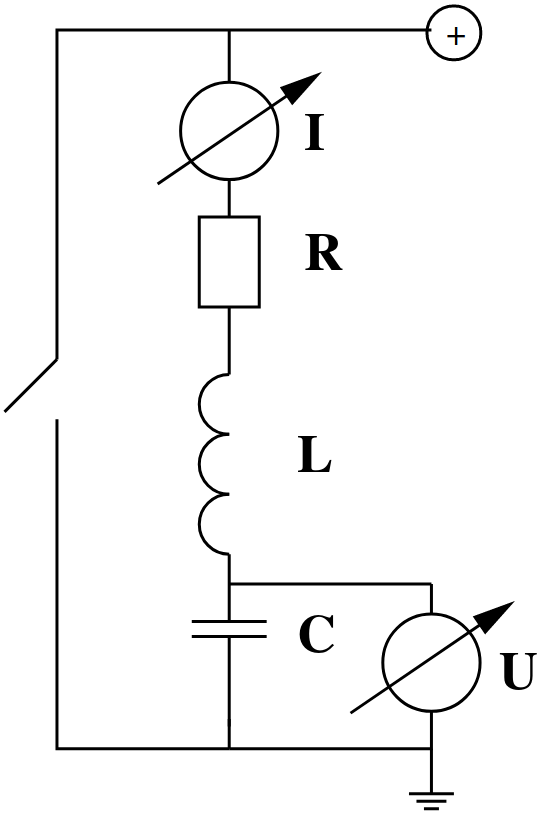
\includegraphics[width = \textwidth]{abbildungen/lcr_schaltbild.png}
\caption{Schaltbild des LCR-Schwingkreises}
\end{figure}
\end{columns}

\end{frame}


\begin{frame}
\frametitle{Lösungen der Differentialgleichung 1}
Bestimmbar über homogene und partikuläre Lösung.
Eigenschaften der Lösung sind abhängig von $\delta$ und $\omega_0$:
\begin{itemize}
\item $\delta < \omega_0$: Schwingfall
\item $\delta = \omega_0$: Aperiodischer Grenzfall
\item $\delta > \omega_0$: Kriechfall
\end{itemize}
\end{frame}

\begin{frame}
\frametitle{Lösungen der Differentialgleichung 2}
\begin{figure}
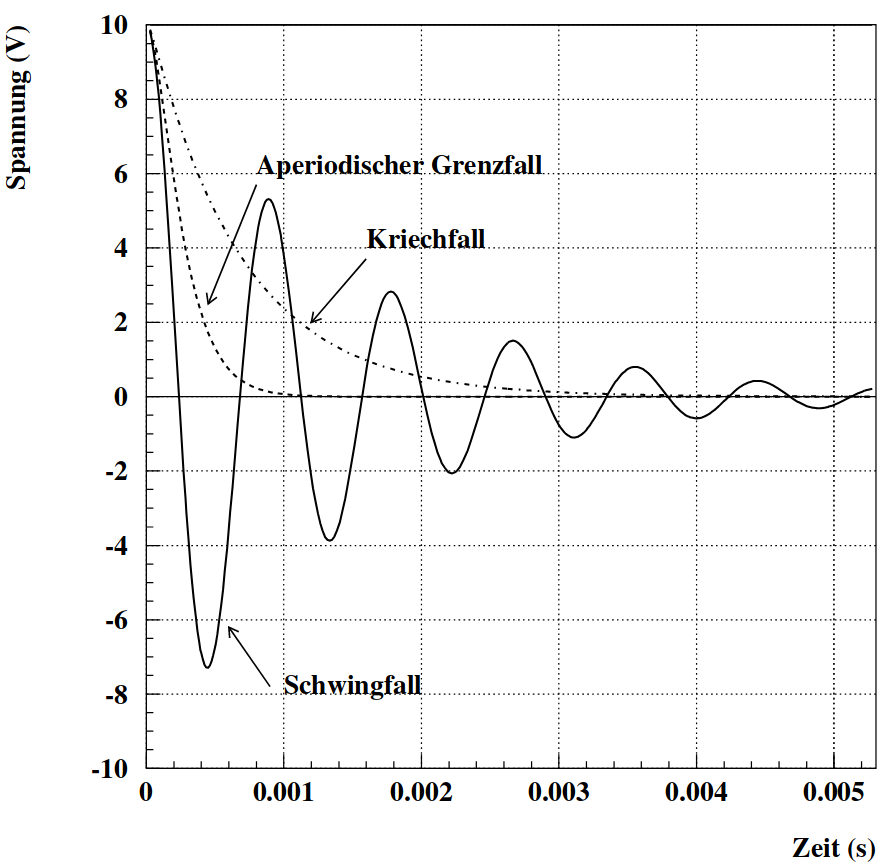
\includegraphics[scale = 0.25]{abbildungen/typen_schwingung.png}
\end{figure}
\end{frame}


\subsection{Versuchsaufbau}

\begin{frame}
\frametitle{Versuchsaufbau}
\begin{figure}
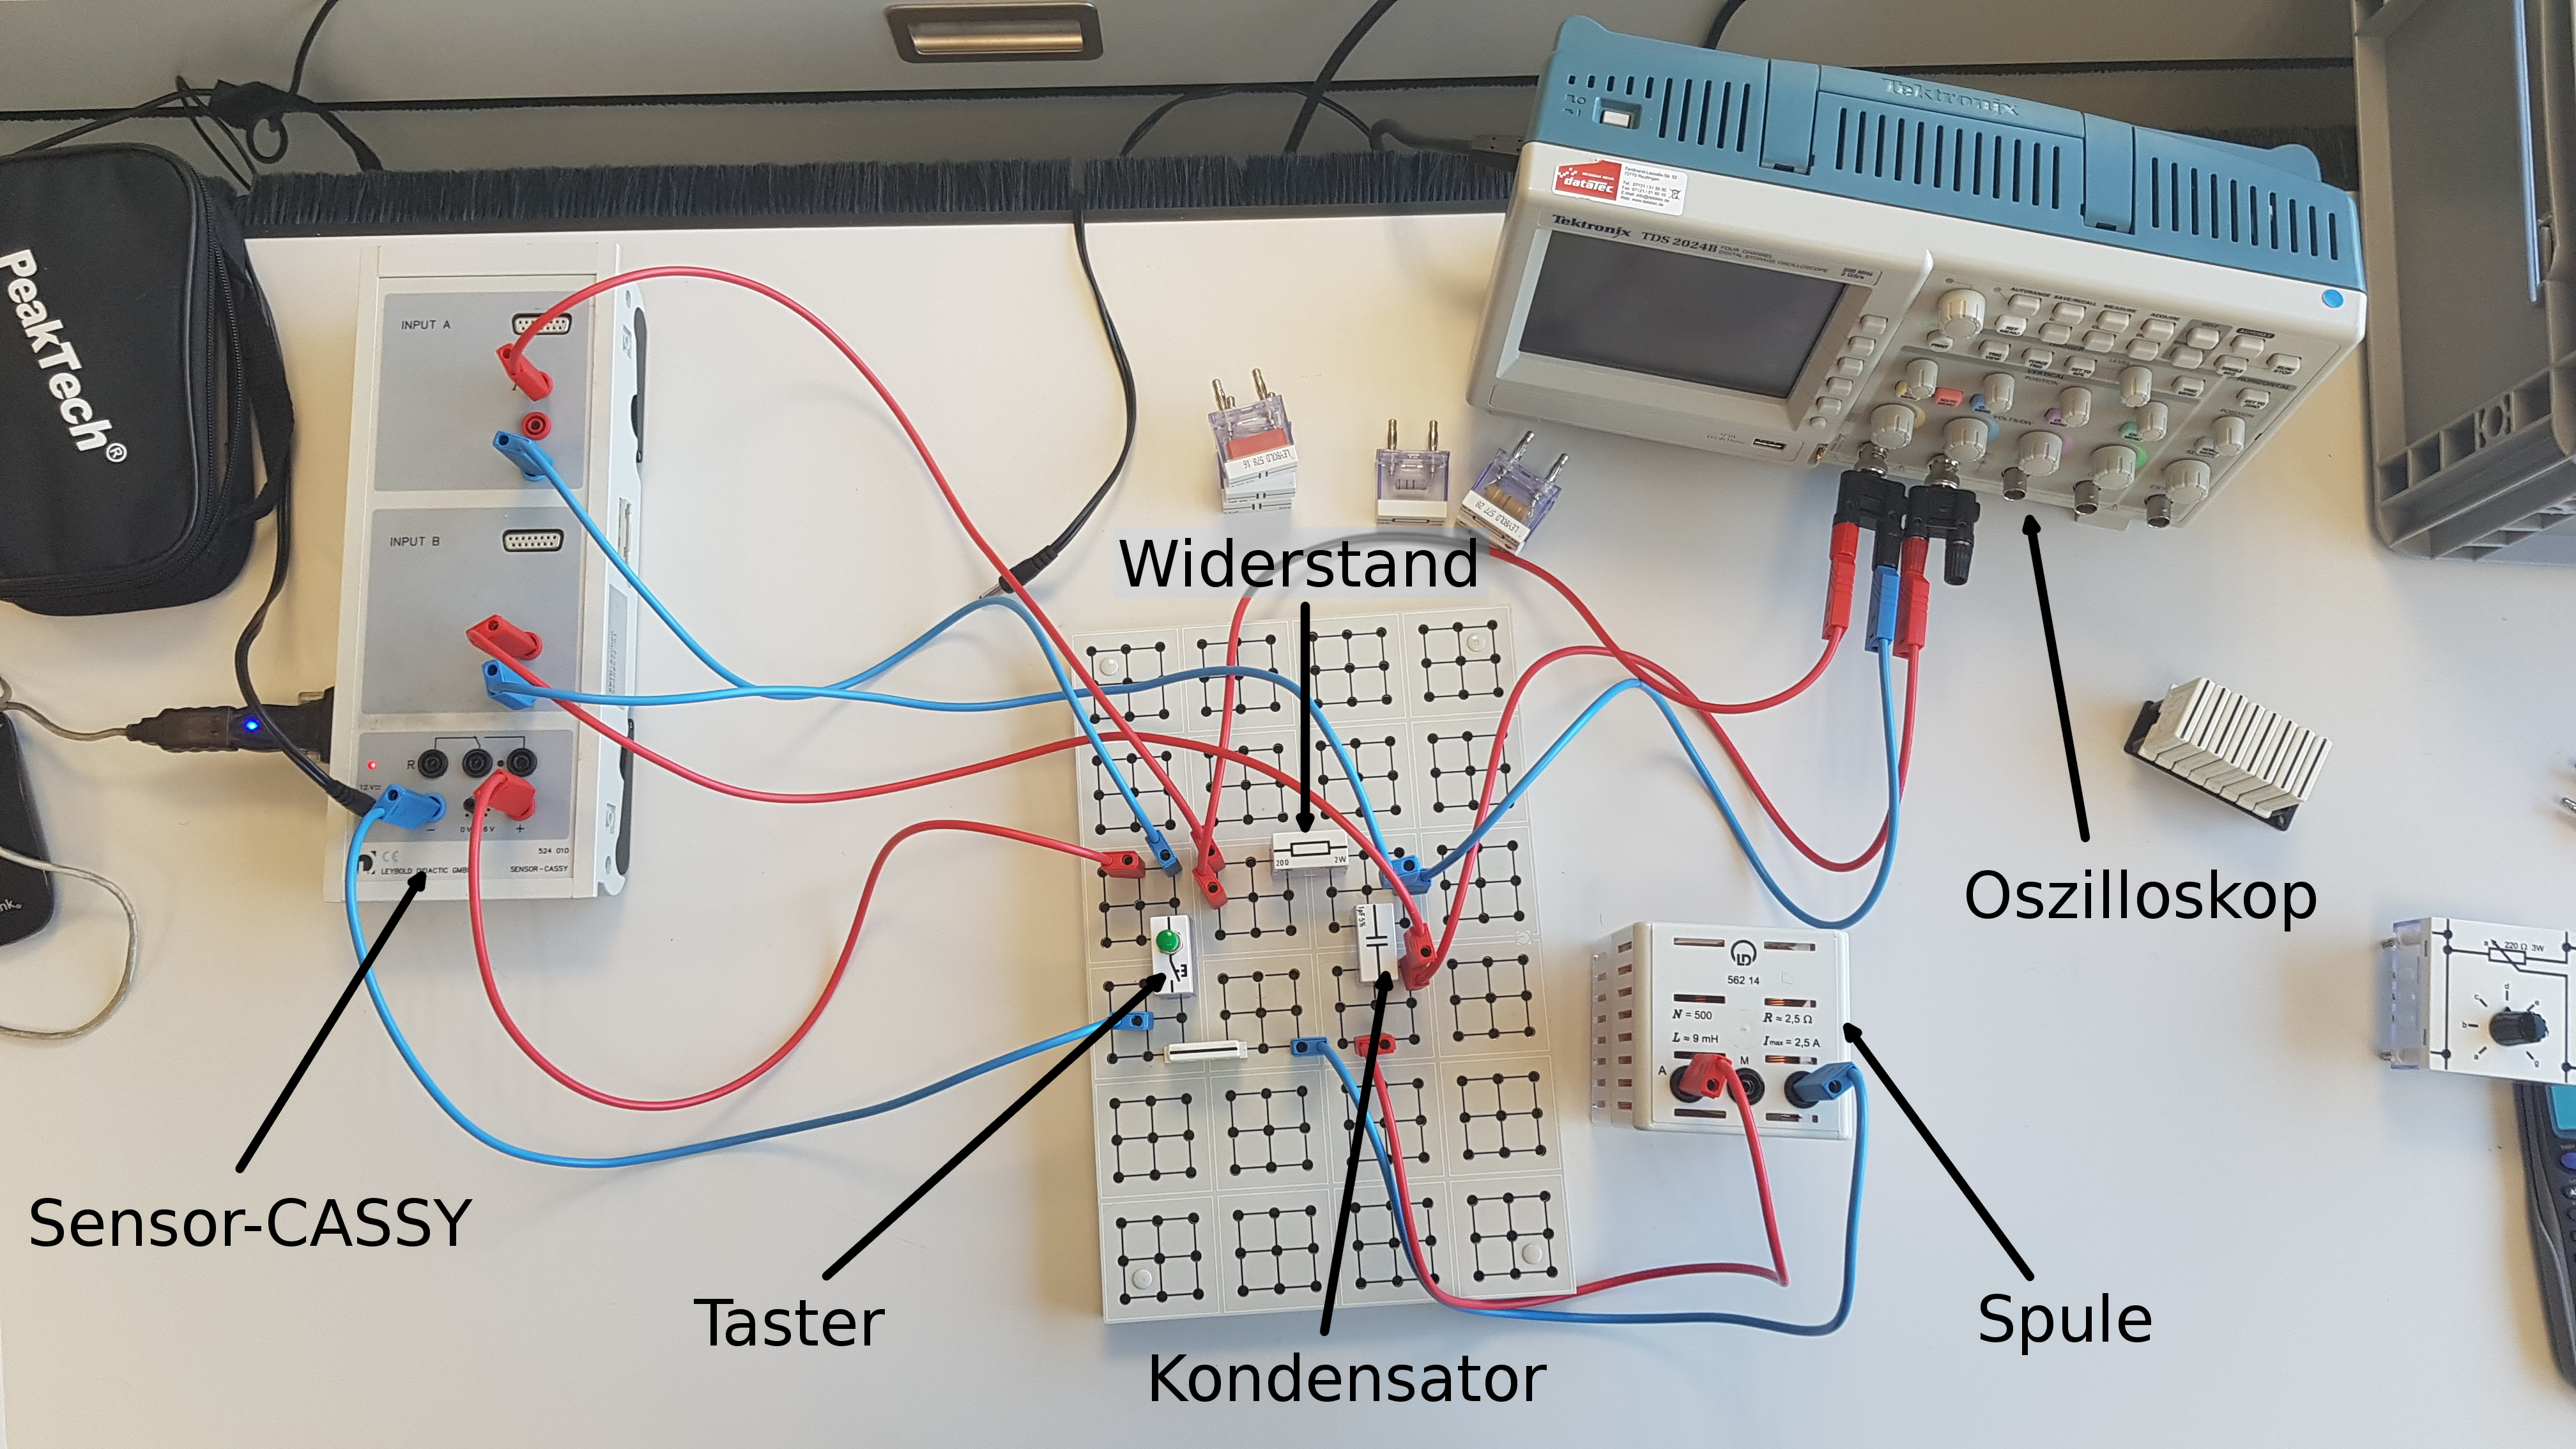
\includegraphics[width=\linewidth]{abbildungen/LCR_aufbau_beschriftet.jpg}
\end{figure}
\end{frame}


\subsection{Versuchsdurchführung}

\begin{frame}
\frametitle{Versuchsdurchführung}

\begin{enumerate}[-]
\item Widerstände unterschiedlicher Größe: 1$\Omega$, 5.1$\Omega$, 10$\Omega$, 20$\Omega$, [47$\Omega$ (nur Gruppe 2)], 100$\Omega$, 1000$\Omega$ und ein Potentiometer
\item Trigger zum Starten der Messreihe
\item 3 Messungen pro Widerstand
\item Messbereich: $\pm$ 3 V (Gruppe 1) oder $\pm$ 10 V (Gruppe 2)
\item Kapazität: 4.7$\mu$F (Gruppe 1) und 0.984$\mu$F (Gruppe 2); Induktivität: 2.24mH (Gruppe 1) und 9mH (Gruppe 2)
\end{enumerate}

\begin{table}
\begin{tabular}{|c|c|c|c|c|}
\hline
\multirow{2}{*}{Messintervall} & \multicolumn{2}{c|}{Anzahl} & \multicolumn{2}{c|}{Messzeit} \\
\cline{2-5}
& Gruppe 1 & Gruppe 2 & Gruppe 1 & Gruppe 2 \\
\hline
10 $\mu$s & 8000 & 2000 & 80 ms & 20 ms \\
\hline
\end{tabular}
\caption{Messparameter}
\end{table}
\end{frame}

\subsection{Versuchsauswertung}

\begin{frame}
\frametitle{Versuchsauswertung}
\begin{figure}
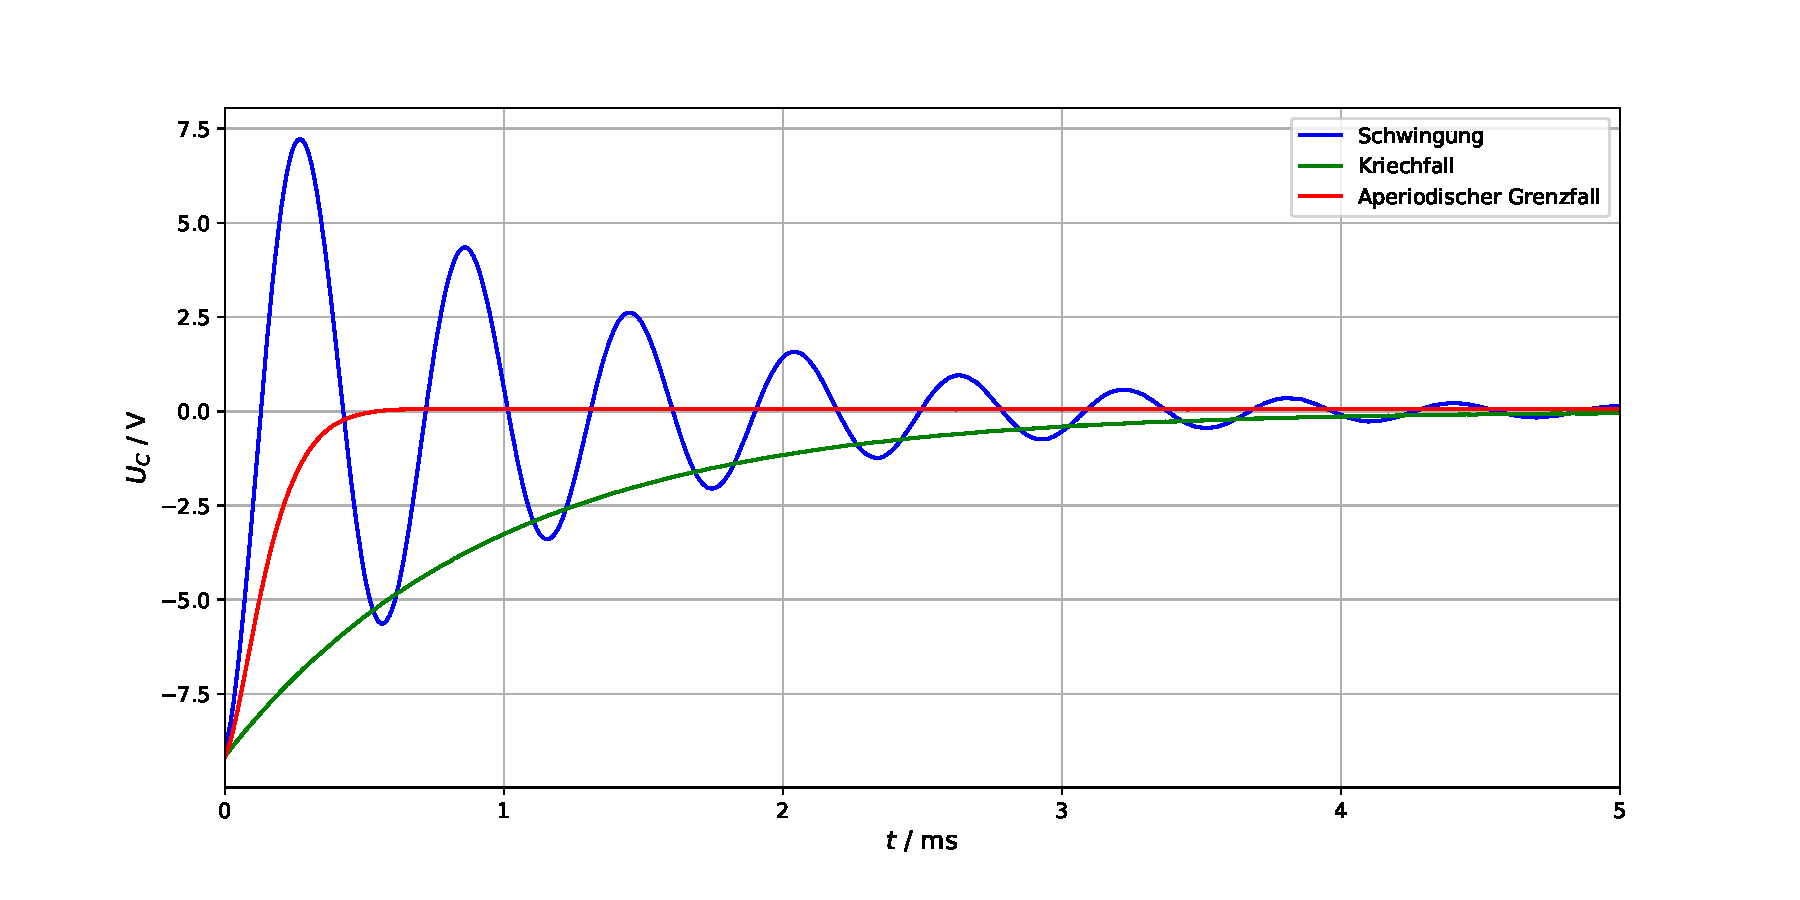
\includegraphics[width=.9\linewidth]{abbildungen/rohdaten.pdf}
\caption{Visualisierung der Schwingung mit einem Widerstand von $10\Omega$, $186\Omega$ und 1k$\Omega$.}
\end{figure}
\end{frame}

%%%%%%%%%%%%%%%%%%%%%%%%%%%%%%%%%%%%%%%%%%%%%%%%%%%%%%%%%%%%%%%%%%

\begin{frame}
\frametitle{Vorgehen bei der Auswertung (1)}
Bestimmung der Kreisfrequenz $\omega$:
\begin{itemize}
\item Peak aus dem Spektrum, das durch eine FFT berechnet wird, bestimmen (Gruppe 1+2)
\item Extrema ablesen und Periodendauer mittels Regression berechnen (Gruppe 2)
\end{itemize}

Bestimmung der Dämpfung $\delta$:
\begin{itemize}
\item mehrere Extrema ablesen und Dämpfung mittels Regression berechnen (Gruppe 2)
\item zwei Extrrema ablesen und Dämpfung mittels Sekantensteigung bestimmen (Gruppe 1)
\item Exponentialfunktion als Einhüllende fitten und Dämpfung aus Modell ablesen (Gruppe 2)
\end{itemize}
\end{frame}

\begin{frame}
\frametitle{FFT - Gruppe 1}
\begin{figure}
\centering
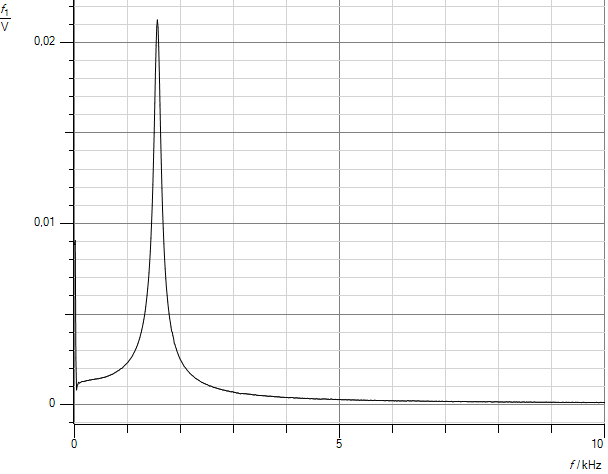
\includegraphics[width=0.7\textwidth]{abbildungen/fft_schwingung_grp1.png}
\caption{FFT-Spektrum des 1$\Omega$ Widerstands der Messung von Gruppe 1. Als Fehler wurde die Auflösung des Spektrums dividiert durch $\sqrt{12}$ verwendet.}
\end{figure}
\end{frame}

\begin{frame}
\frametitle{FFT - Gruppe 2}
\begin{figure}
\centering
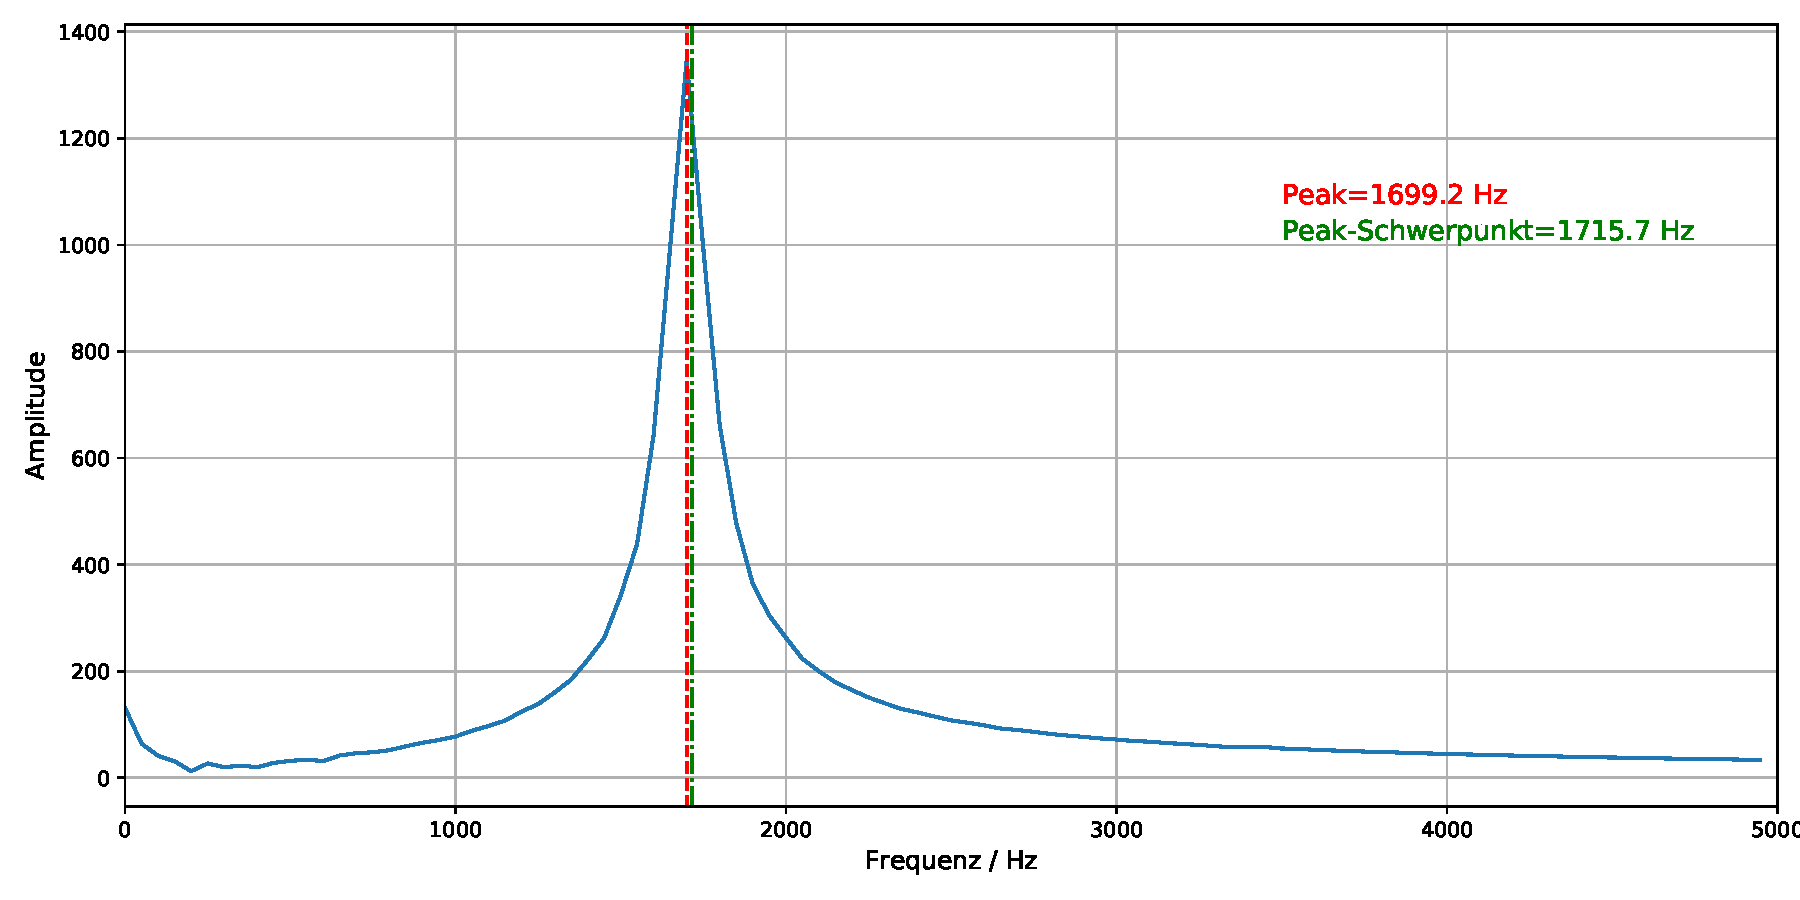
\includegraphics[width=0.9\textwidth]{abbildungen/fft_schwingung_grp2.pdf}
\caption{FFT-Spektrum des 1$\Omega$ Widerstands der Messung von Gruppe 2. Die rote Linie markiert das Argument-Maximum während die grüne Linie das Resultat der Peakfinder-Methode visualisiert. Als Fehler wurde die Differenz beider Werte verwendet.}
\end{figure}
\end{frame}

\begin{frame}
\frametitle{Regressionen - Gruppe 2}
\begin{figure}
\centering
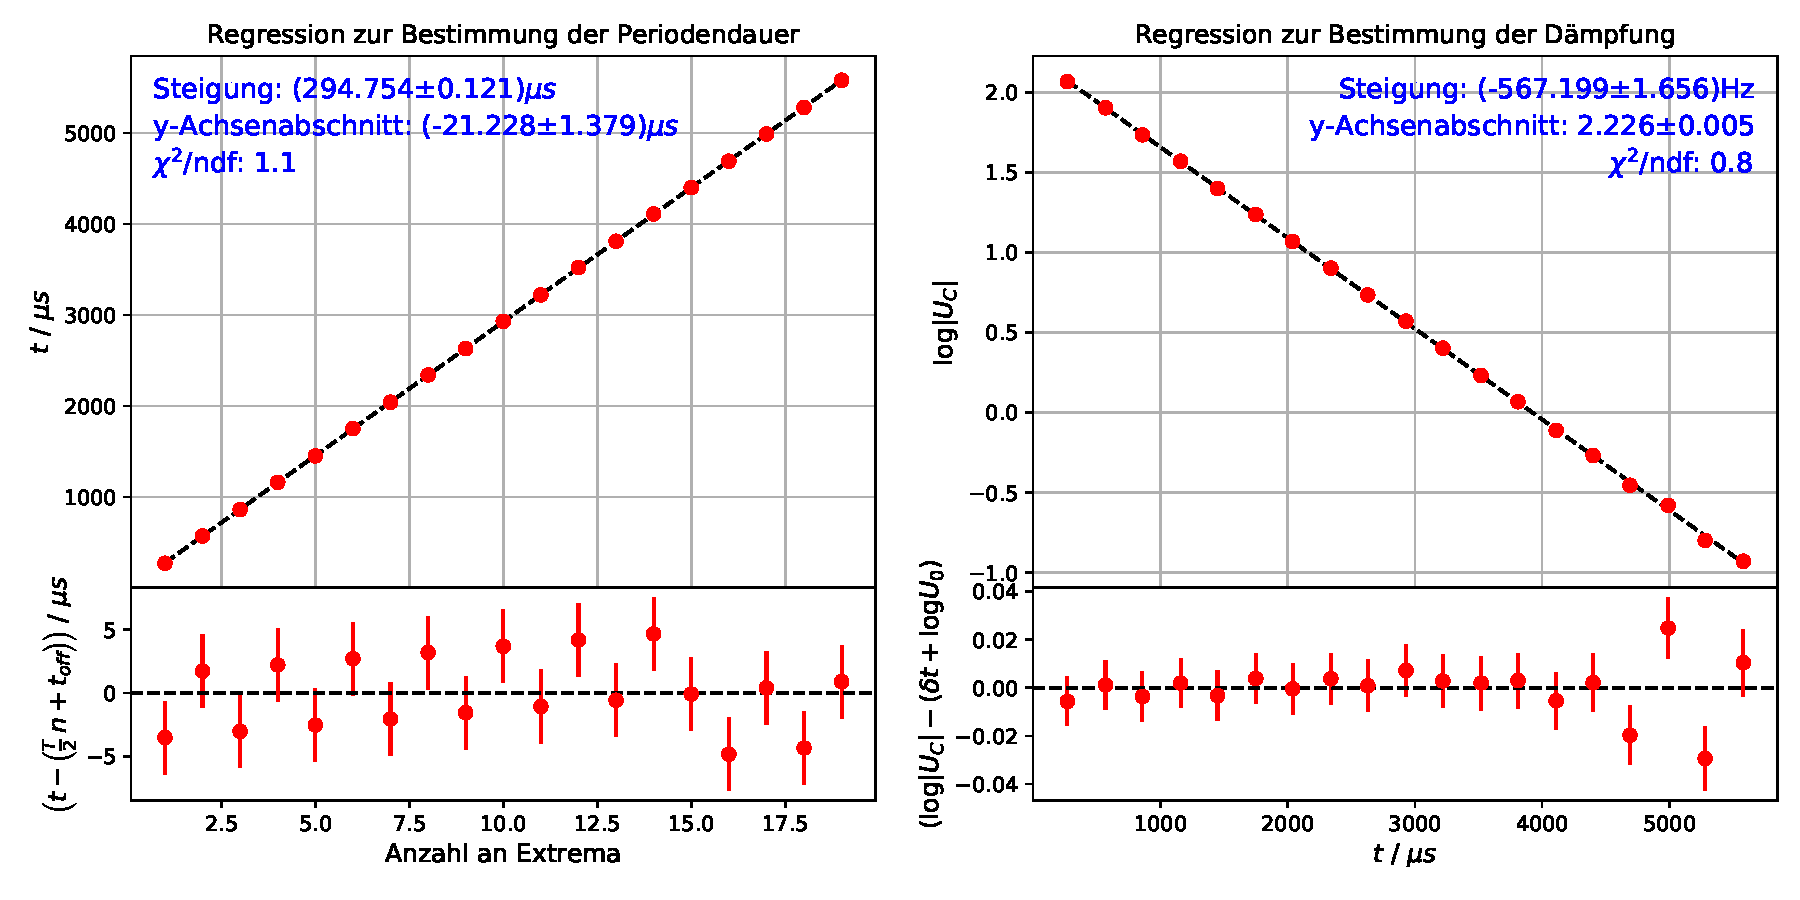
\includegraphics[width=0.9\textwidth]{abbildungen/reg_schwingung_grp2.pdf}
\caption{Regressionen für eine Messung des 5.1$\Omega$ Widerstands von Gruppe 2. Als Fehler auf $U_C$ und $t$ wurde die Auflösung verwendet.}
\end{figure}
\end{frame}

\begin{frame}
\frametitle{Exp-Einhüllende - Gruppe 2}
\begin{figure}
\centering
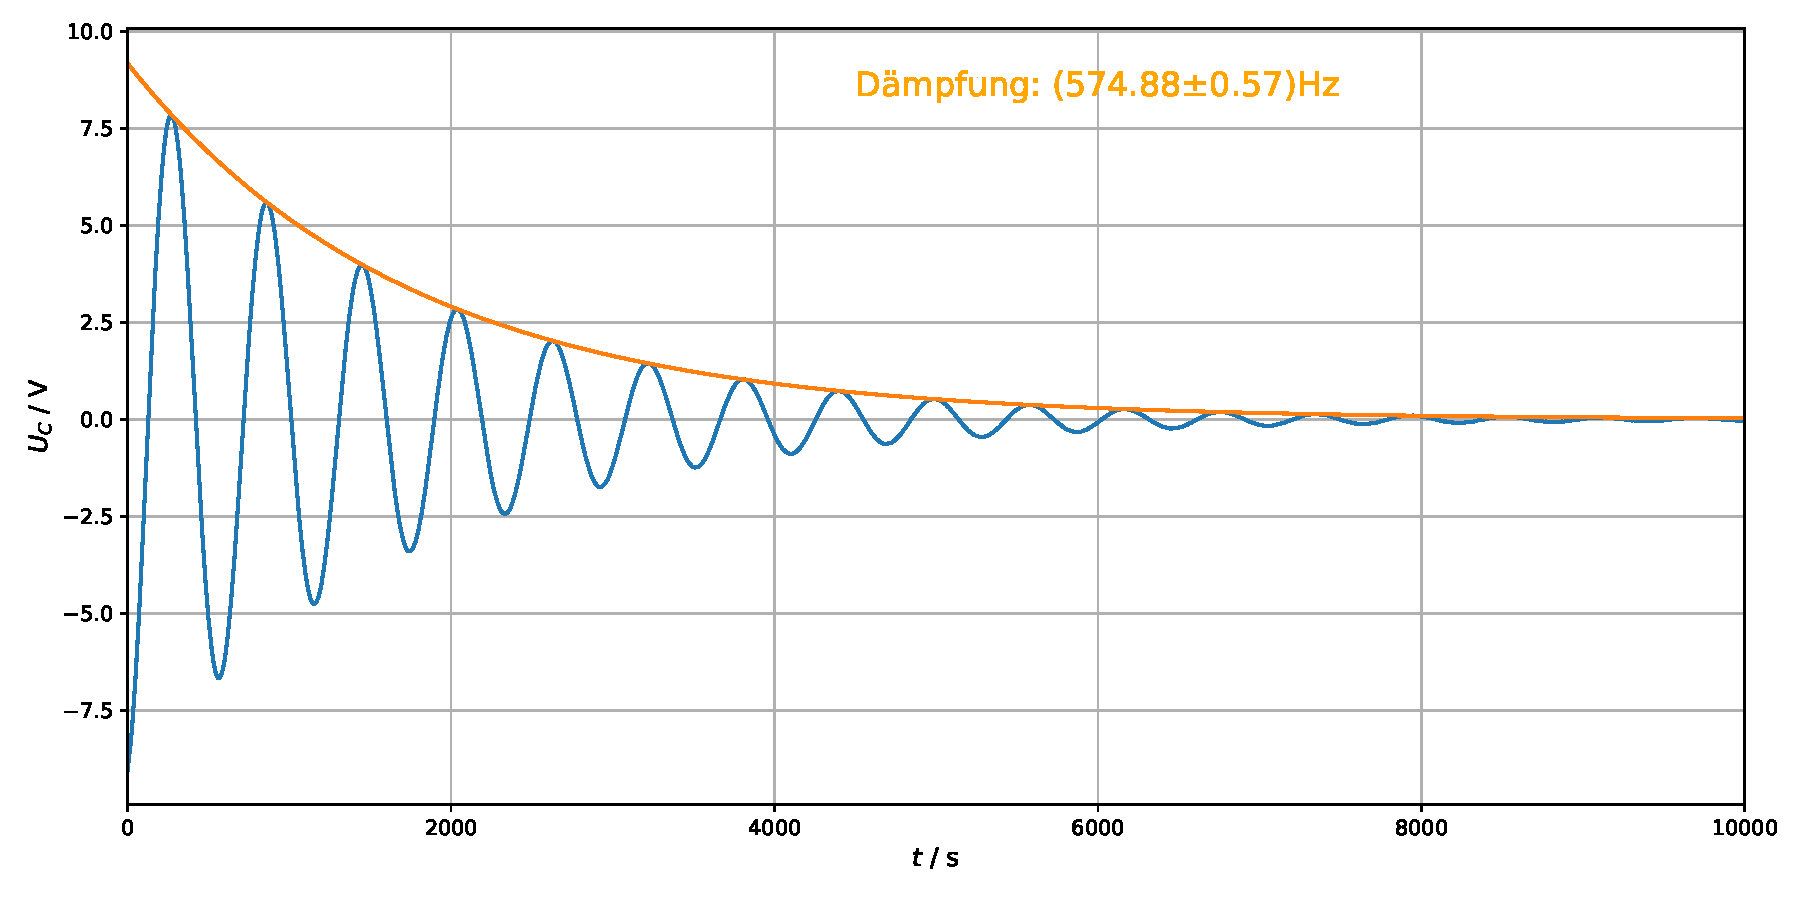
\includegraphics[width=0.9\textwidth]{abbildungen/exp_grp2.pdf}
\caption{Exponentiell Einhüllende für eine Messung des 5.1$\Omega$ Widerstands von Gruppe 2.}
\end{figure}
\end{frame}


\begin{frame}
\frametitle{Frequenzen und Dämpfungen - Gruppe 1}
\begin{figure}
\centering
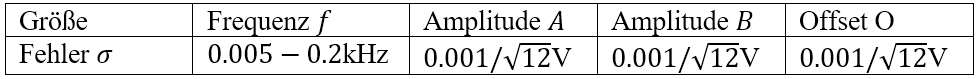
\includegraphics[width=0.9\textwidth]{abbildungen/1VFehler.PNG}
\caption{Einzelfehler der 1. Gruppe.}
\end{figure}

\begin{figure}
\centering
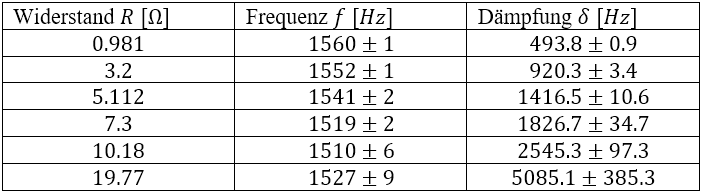
\includegraphics[width=0.9\textwidth]{abbildungen/1VWerte.PNG}
\caption{Ergebnisse der 1. Gruppe.}
\end{figure}
\end{frame}

\begin{frame}
\frametitle{Frequenzen und Dämpfungen - Gruppe 2}
\begin{table}
\centering
\begin{tabular}{c|c|c}
Ohmscher Widerstand / $\Omega$ & Frequenz / Hz & Dämpfung / Hz \\
\hline
$1$ & $1696.9 \pm 0.6$ & $331.32\pm 7.38$ \\
$5.1$ & $1696.3 \pm 0.7$ & $570.61\pm 4.34$ \\
$10$ & $1695.1 \pm 1.0$ & $854.48\pm 2.76$ \\
$20$ & $1689.2 \pm 2.1$ & $1412.21\pm 2.57$  \\
$47$ & $1628.6 \pm 4.8$ & $2923.66\pm 29.28$
\end{tabular}
\caption{Mit Regression ermittelte Frequenzwerte und durch die exponentiell Einhüllende bestimmte Dämpfungen von Gruppe 2.}
\end{table}
\end{frame}

%%%%%%%%%%%%%%%%%%%%%%%%%%%%%%%%%%%%%%%%%%%%%%%%%%%%%%%%%%%%%%%%%%%%%%%%%%%%%%%%%

\begin{frame}
\frametitle{Vorgehen bei der Auswertung (2)}
Bestimmung von Restwiderstand $R_0$ und Induktivität $L$ mittels Regression von $\delta$ über $R$ (Gruppe 1+2) \\
\ \\
Bestimmung der Grundfrequenz $\omega_0$:
\begin{itemize}
\item durch Korrektur von $\omega$ mit $\delta$ (Gruppe 1)
\item mittels Regresion von $\omega^2$ über $\delta^2$ bei festgesetzter Steigung von $-1$ (Gruppe 2)
\end{itemize} 
\ \\
\ \\
Alternativ: Mit vorher berechnetem $R_0$ mittels Regresssion von $\omega^2$ über $(R+R_0)^2$ die Induktivität $L$ und Kreisfrequenz $\omega_0$ bestimmen (Gruppe 2) \\
\ \\
Kapazität $C$ aus $\omega_0$ und $L$ berechnen (Gruppe 1+2)

\end{frame}

\begin{frame}
\frametitle{$\delta$ über R - Gruppe 1}
\begin{figure}
\centering
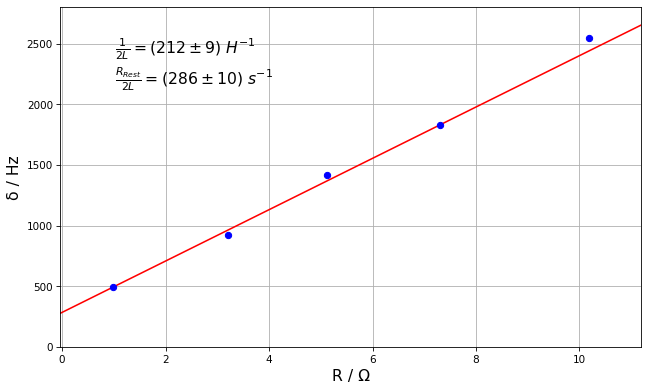
\includegraphics[width=0.85\textwidth]{abbildungen/LCRegression.png}
\caption{Regression von $\delta$ über R mit den Frequenz- und Dämpfungswerten der Gruppe 1.}
\end{figure}

\end{frame}


\begin{frame}
\begin{figure}
\centering
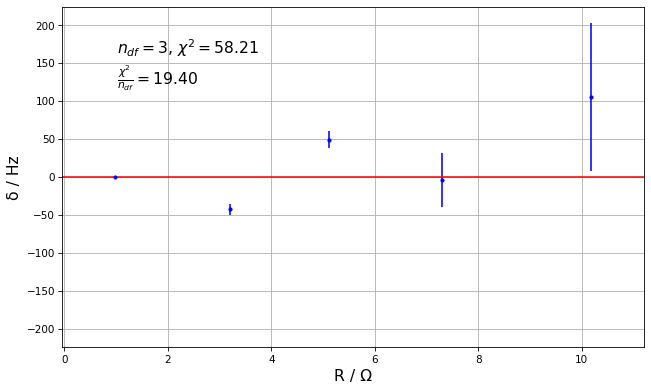
\includegraphics[width=0.7\textwidth]{abbildungen/LCResiduen.png}
\caption{Residuen der Regression von $\delta$ über R mit den Frequenz- und Dämpfungswerten der Gruppe 1.}
\end{figure}
Es ergibt sich $L = 2.363 \pm 0.096$mH, da für die Steigung $\Delta = \frac{1}{2L}$ gilt.
\end{frame}

\begin{frame}
Mit den durch $\omega_0^2 = \omega^2 + \delta^2$ korrigierten Kreisfrequenzen und dem Zusammenhang $\omega_0 = \frac{1}{\sqrt{LC}}$ lässt sich die Kapazität durch 
$$ C = \frac{1}{(\omega^2 + \delta^2) L}$$
bestimmen:

\begin{figure}
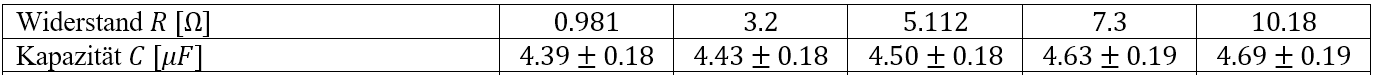
\includegraphics[width = \textwidth]{abbildungen/1VCWerte_mod.PNG}
\end{figure}
\end{frame}


\begin{frame}
\frametitle{$\delta$ über R - Gruppe 2}
\begin{figure}
\centering
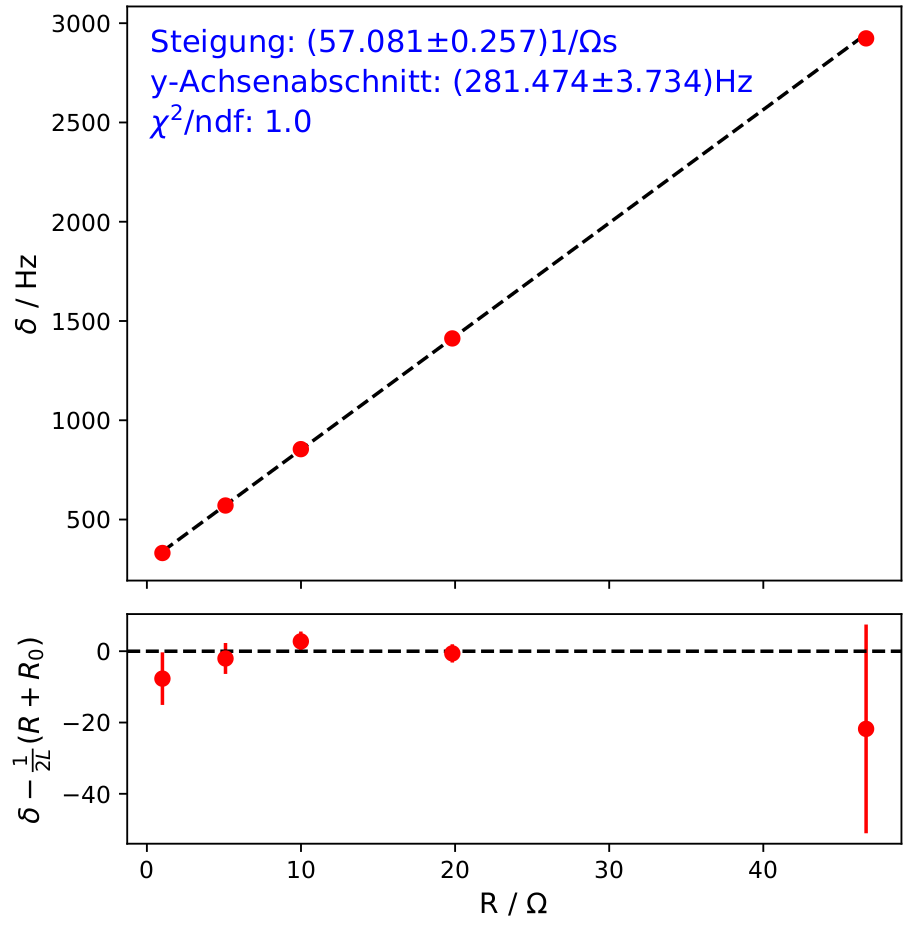
\includegraphics[width=0.4\textwidth]{abbildungen/reg_delR.png}
\caption{Regression von $\delta$ über R mit den Frequenz- und Dämpfungswerten der Gruppe 2.}
\end{figure}
Es ergibt sich $R_0 = 4.94\pm 0.07\Omega$ durch Division des y-Achsenabschnitts mit der Steigung.
\end{frame}

\begin{frame}
\frametitle{$\omega^2$ über $(R+R_0)^2$ - Gruppe 2}
\begin{figure}
\centering
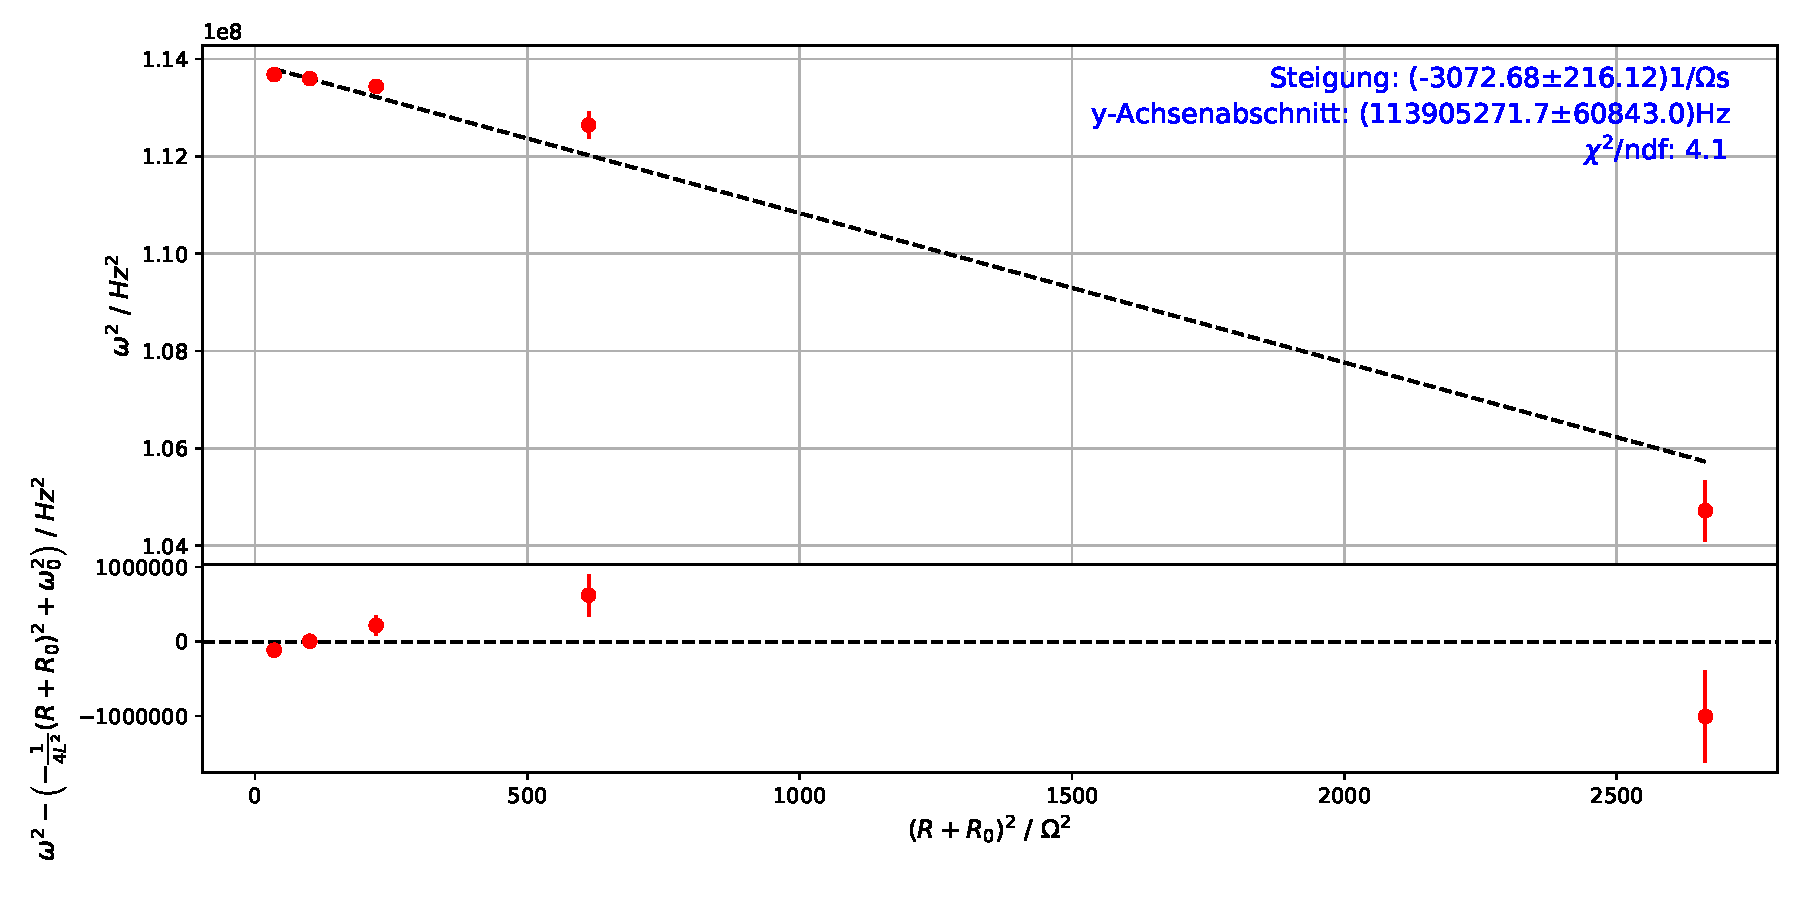
\includegraphics[width=0.8\textwidth]{abbildungen/reg_Rome.pdf}
\caption{Regression von $\omega^2$ über $(R+R_0)^2$ der Gruppe 2 zur Bestimmung von $L$ und $\omega_0$.}
\end{figure}
Daraus folgt $\omega_0 = (10672.64\pm2.85)$Hz und $L=(9.020 \pm 0.317)$mH. Damit ist $C = (0.973 \pm 0.034)\mu$F.
\end{frame}


%%%%%%%%%%%%%%%%%%%%%%%%%%%%%%%%%%%%%%%%%%%%%%%%%%%%%%%%%%%%%%%%%%%%%%%%%%%%%%%%%%


\subsection{Fazit}

\begin{frame}
\frametitle{Fazit (1)}
Gruppe 1:
\begin{figure}
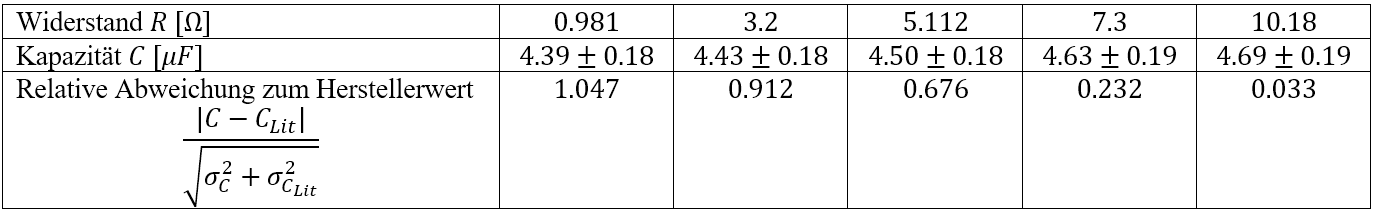
\includegraphics[width=\textwidth]{abbildungen/1VCWerte.PNG}
\end{figure}
Gruppe 2:
\begin{table}
\begin{adjustbox}{width = \textwidth}
\begin{tabular}{c|c|c|c|c}
& Induktivität / mH & rel. Abweichung & Kapazität / $\mu$H & rel. Abweichung \\
\hline
Methode 1 (s.o.) & $9.020 \pm 0.317$ & 0.03 & $0.973 \pm 0.034$ & 0.32 \\
Methode 2 & $8.759\pm0.079$ & 1.89 & $1.002 \pm 0.009$ & 1.98 
\end{tabular}
\end{adjustbox}
\end{table}
\end{frame}

\begin{frame}
\frametitle{Fazit (2)}
Die Einstellung des aperiodischen Grenzfalls ergab folgende Werte:
\begin{table}
\begin{tabular}{c|cc|c}
Gruppe & $R_{gemessen}$ / $\Omega$ & $R_{erwartet}$ / $\Omega$ & relative Abweichung \\
\hline
1 & $40.45 \pm 0.08$ & $43.66\pm 1.12$ & 2.85 \\
2 & $190.93 \pm 1$ & $191.27 \pm 0.11$ & 0.34
\end{tabular}
\end{table}
\end{frame}

\section{Gekoppelte LC-Schwingkreis}

\begin{frame}
\centering
\Large{Gekoppelte LC-Schwingkreise}
\end{frame}

\subsection{Theorie}

\begin{frame}
\frametitle{Die Differentialgleichung der gekoppelten LC-Schwingkreise}
\begin{figure}
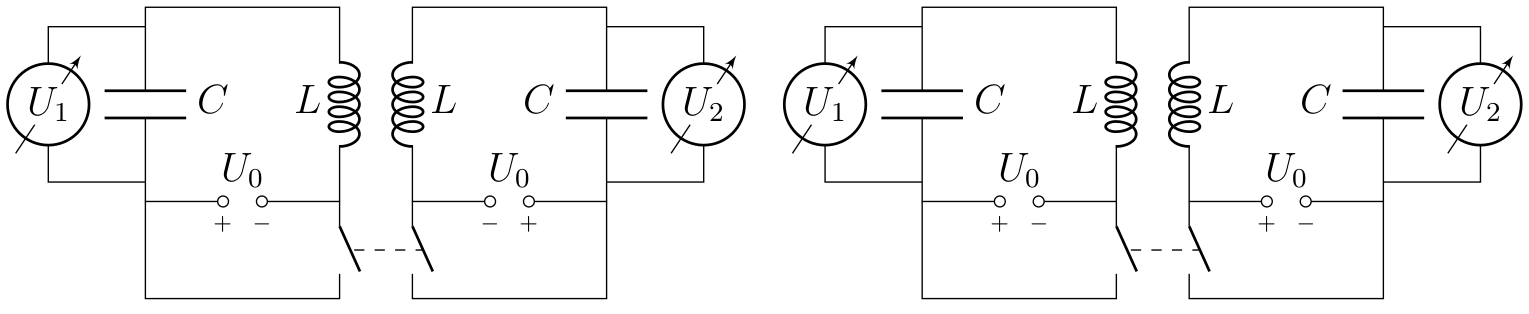
\includegraphics[width = \textwidth]{abbildungen/theorie_LC.png}
\end{figure}

Das System wird durch das folgende DGL-System beschrieben:
$$\ddot{I_1} + k \ddot{I_2} + \frac{1}{LC} I_1 = 0$$\ \\
$$\ddot{I_2} + k \ddot{I_1} + \frac{1}{LC} I_2 = 0$$
mit Kopplungsgrad $k\in (0,1)$. Die tatsächlich gemessen Kreisfrequenzen sind durch $k$ beeinflusst.
\end{frame}

\subsection{Versuchsaufbau}

\begin{frame}
\frametitle{Versuchsaufbau - Schwebung}
\begin{figure}
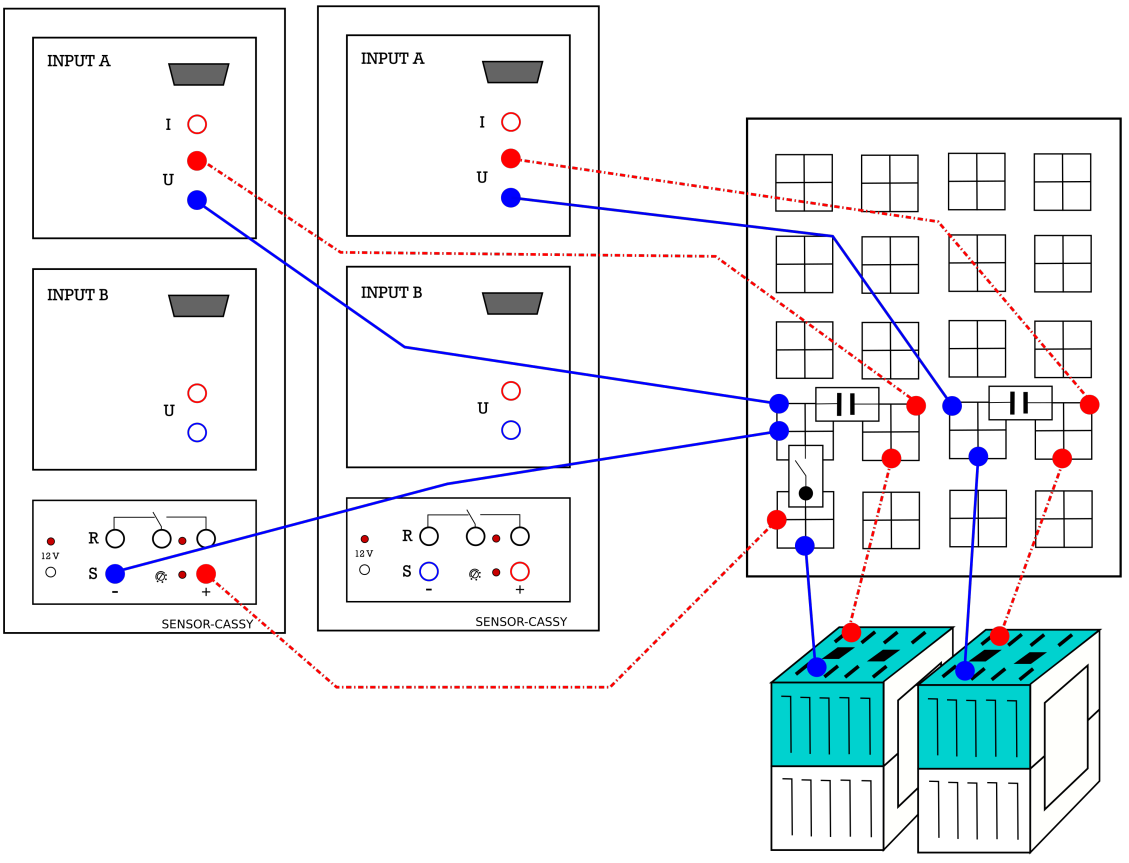
\includegraphics[width=0.6\linewidth]{abbildungen/aufbau_LC.png}
\caption{Aufbau zur Messung einer Schwebung.}
\end{figure}
\end{frame}

\begin{frame}
\frametitle{Versuchsaufbau - gleich- und gegensinnige Schwingung}
\begin{figure}
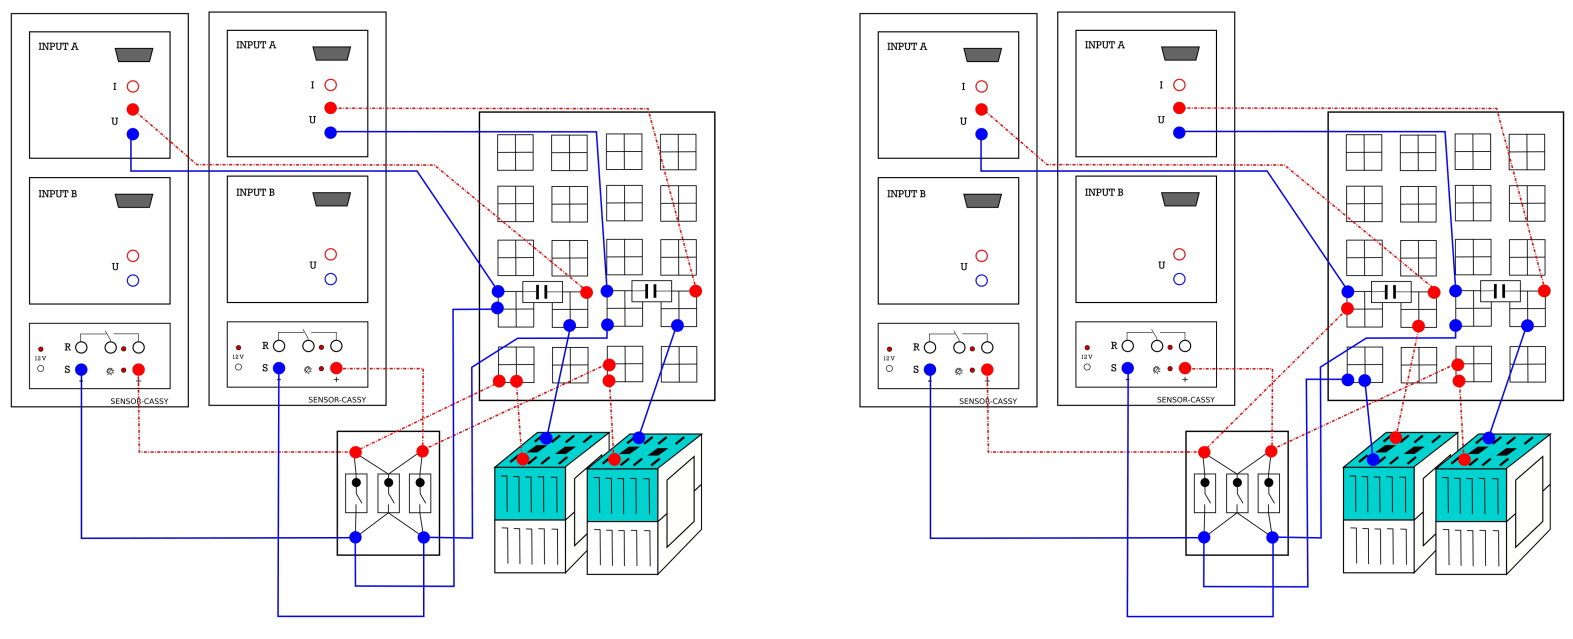
\includegraphics[width=\linewidth]{abbildungen/aufbau_LC_gg.png}
\caption{Aufbau zur Messung einer gleich- bzw. gegensinniger Schwingung.}
\end{figure}
\end{frame}

\begin{frame}
\frametitle{Versuchsdurchführung}
Folgende Messparameter wurden verwendet:
\begin{table}
\begin{tabular}{|c|c|c|c|c|}
\hline
\multirow{2}{*}{Messintervall} & \multicolumn{2}{c|}{Anzahl} & \multicolumn{2}{c|}{Messzeit} \\
\cline{2-5}
& Gruppe 1 & Gruppe 2 & Gruppe 1 & Gruppe 2 \\
\hline
10 $\mu$s & 2000 & 8000 & 20 ms & 80 ms \\
\hline
\end{tabular}
\end{table}

\begin{enumerate}[-]
\item Trigger zum Starten der Messreihe
\item Bei der Schwebungsmessungen wurden unterschiedliche Abstände und der Aufbau mit Eisenkern gemessen.
\item Messbereich: $\pm$ 3 V (Gruppe 1) oder $\pm$ 10 V (Gruppe 2)
\item Gruppe 1: Kapazität: 1.002$\mu$F und 1.000$\mu$F; Induktivität: 2.240mH und 2.223mH
\item Gruppe 2: Kapazität: 0.984$\mu$F und 0.980$\mu$F; Induktivität 9.00mH und 9.03mH
\end{enumerate}

\end{frame}

\subsection{Schwebung}
\begin{frame}
\centering
\Large{Schwebung}
\end{frame}


\begin{frame}
\frametitle{Rohdaten - Gruppe 1}
\begin{figure}
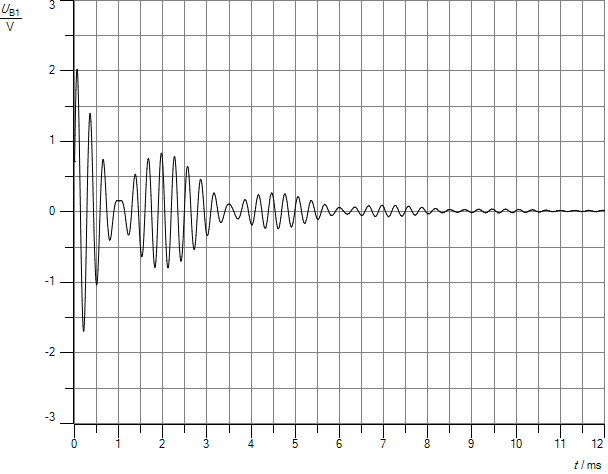
\includegraphics[width = .7\framewidth]{abbildungen/plotsLC/Schwebung.png}
\caption{Spannungswerte der Schwebungsmessung ohne Eisenkern von Gruppe 1 im Zeitbereich.}
\end{figure}
\end{frame}


\begin{frame}
\frametitle{FFT - Gruppe 1}
\begin{figure}
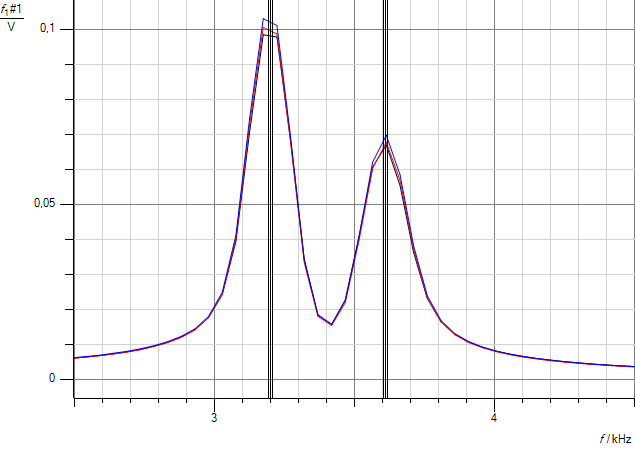
\includegraphics[width = .65\framewidth]{abbildungen/plotsLC/FFTFehler.png}
\caption{Frequenzspektrum der Spannungswerte der Schwebungsmessung ohne Eisenkern von Gruppe 1.}
\end{figure}
\end{frame}

\begin{frame}
\frametitle{Rohdaten - Gruppe 2}
\begin{figure}
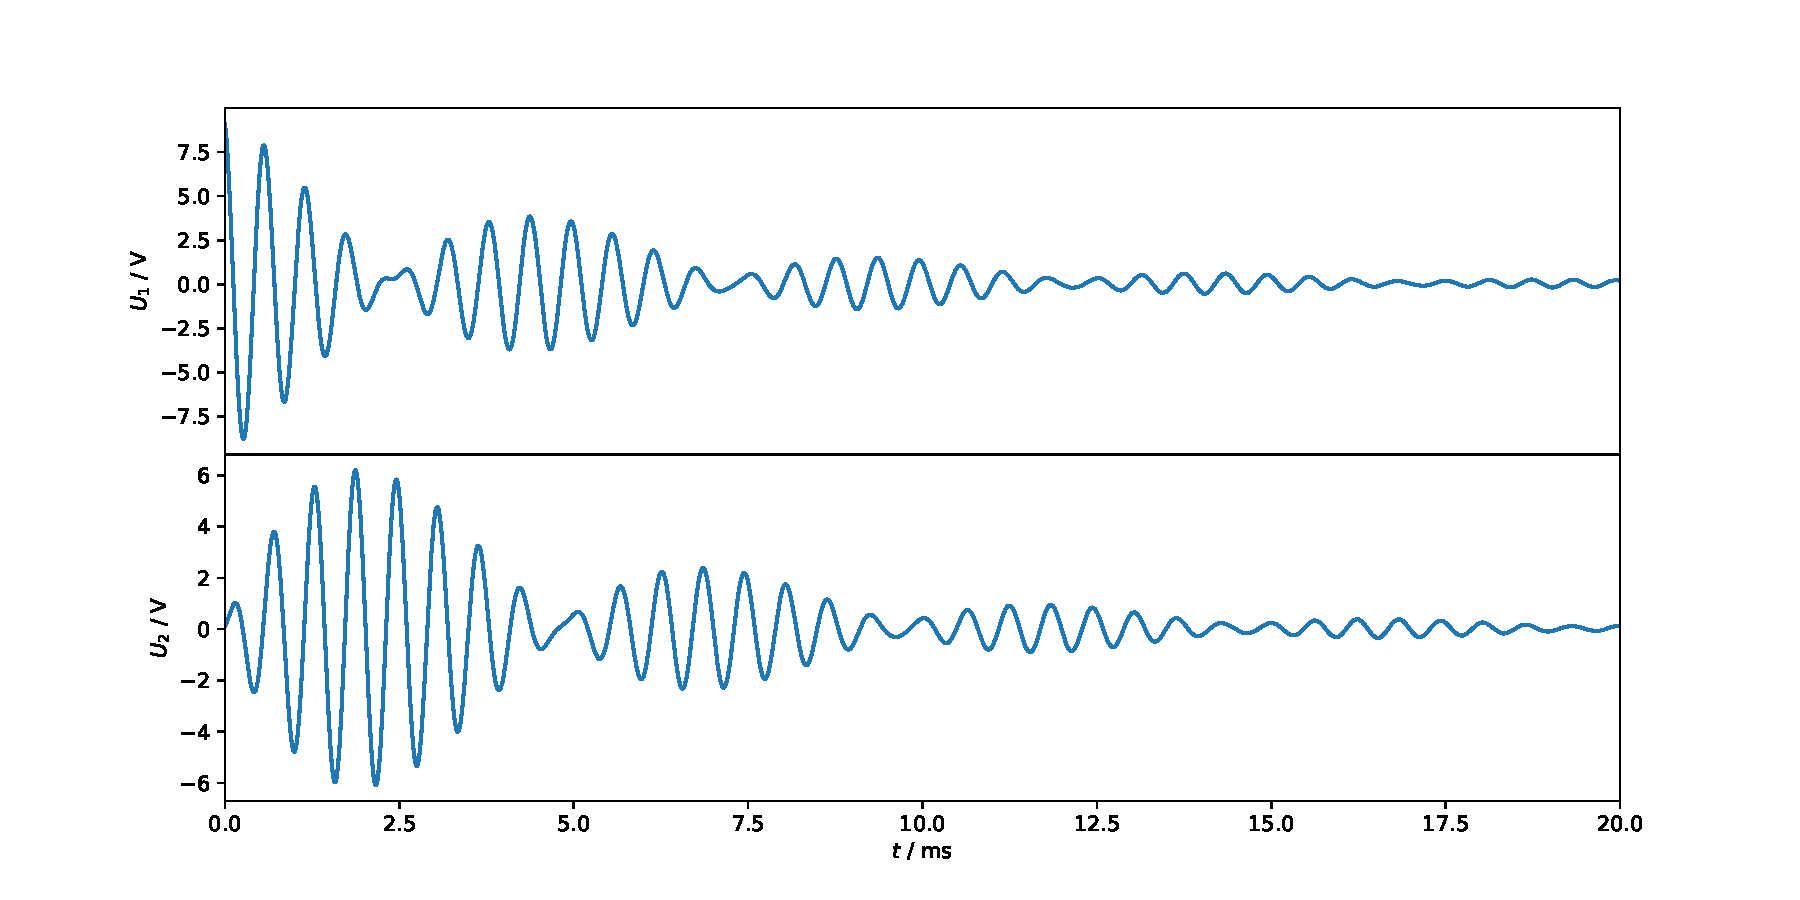
\includegraphics[width = \framewidth]{abbildungen/plotsLC/schwebung_roh.pdf}
\caption{Spannungswerte einer Schwebungsmessung von Gruppe 2 im Zeitbereich.}
\end{figure}
\end{frame}

\begin{frame}
\frametitle{FFT - Gruppe 2}
\begin{figure}
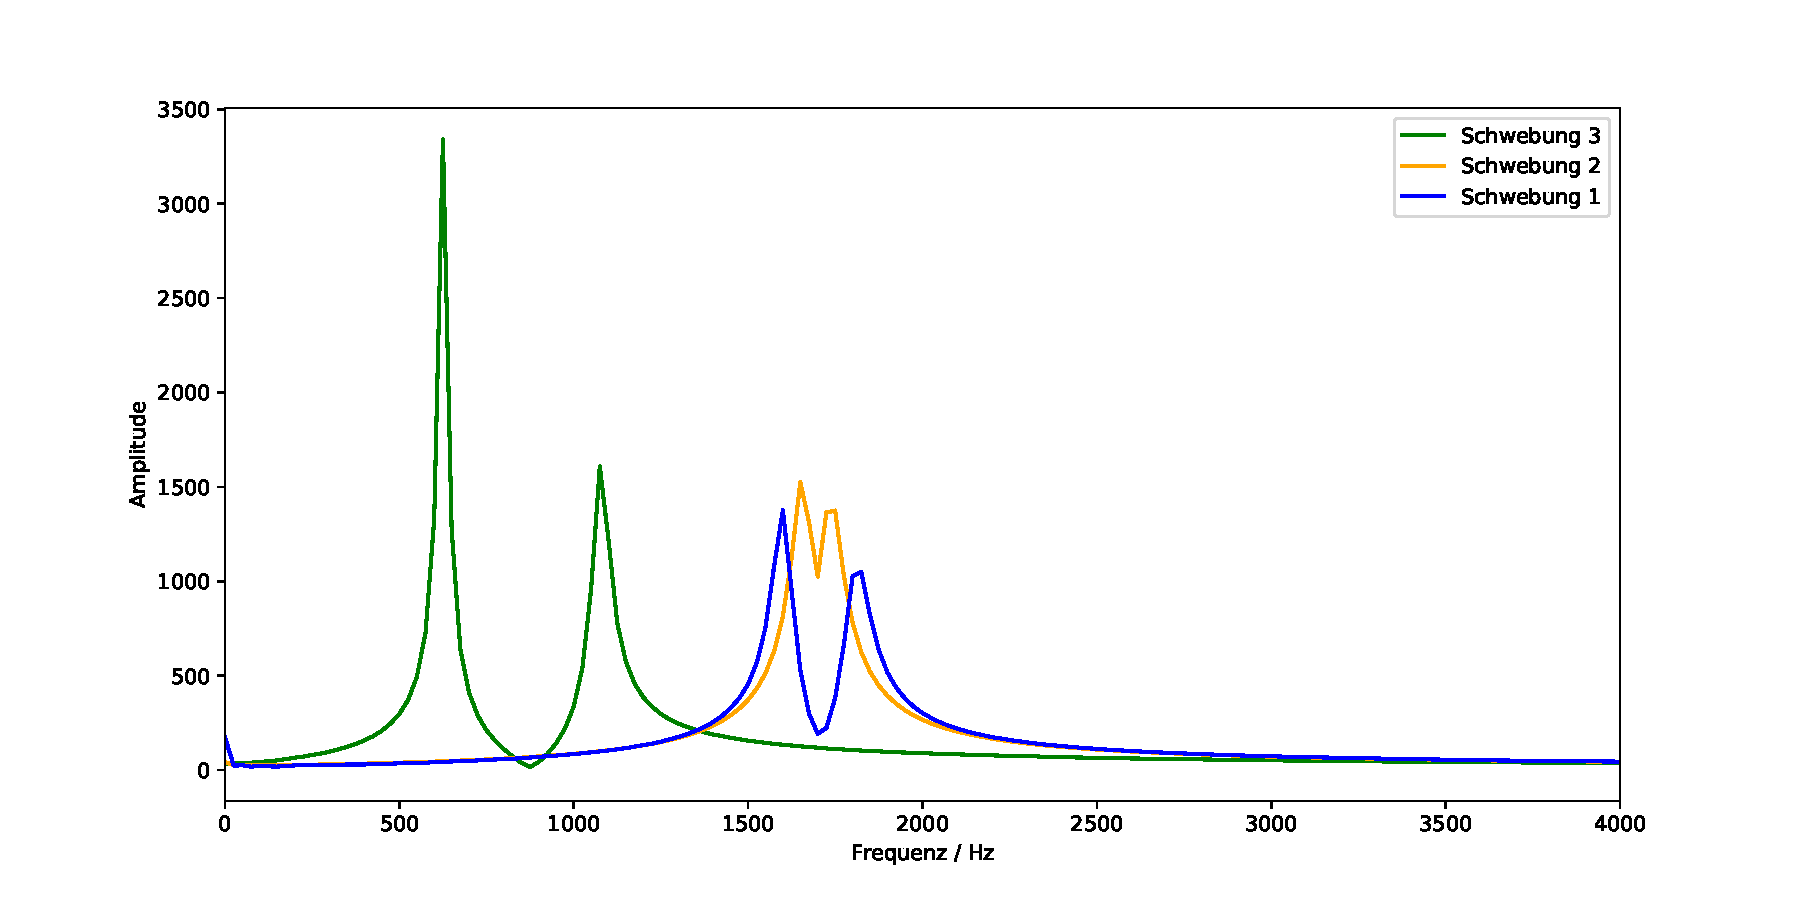
\includegraphics[width = \framewidth]{abbildungen/plotsLC/FFT_schwebungen.pdf}
\caption{Frequenzspektrum der Spannungswerte aller Schwebungsmessung von Gruppe 2.}
\end{figure}
\end{frame}

\begin{frame}
\frametitle{Ergebnisse}

\begin{table}
\begin{adjustbox}{width=\textwidth}
\begin{tabular}{|c|c|c|c|c|}
\hline
\multirow{2}{*}{\ } & \multicolumn{2}{c|}{Fundamentalfrequenzen / Hz} & \multicolumn{2}{c|}{Kopplungsgrad} \\
\cline{2-5}
 & Gruppe 1 & Gruppe 2 & Gruppe 1 & Gruppe 2 \\
\hline
ohne Eisenkern & $3198\pm10$, $3621\pm10$ & $1598.7 \pm 1$, $1832.1 \pm 7.5$ & $0.121\pm 0.004$ & $0.1355 \pm 0.0041$ \\
mit Eisenkern & $1247\pm10$, $2130\pm10$ & $631.8 \pm 6.9$, $1094 \pm 19$ & $0.489\pm 0.006$ & $0.4999 \pm 0.0155$ \\
\hline
\end{tabular}
\end{adjustbox}
\end{table}

Mit Eisenkern wird ein Kopplungsgrad von $\approx 0.5$ erwartet.
\end{frame}

\subsection{Gleich- und gegensinnige Schwingung}
\begin{frame}
\centering
\Large{Gleich- und gegensinnige Schwingung}
\end{frame}

\begin{frame}
\frametitle{Gegensinnige - Zeitbereich}
\begin{figure}
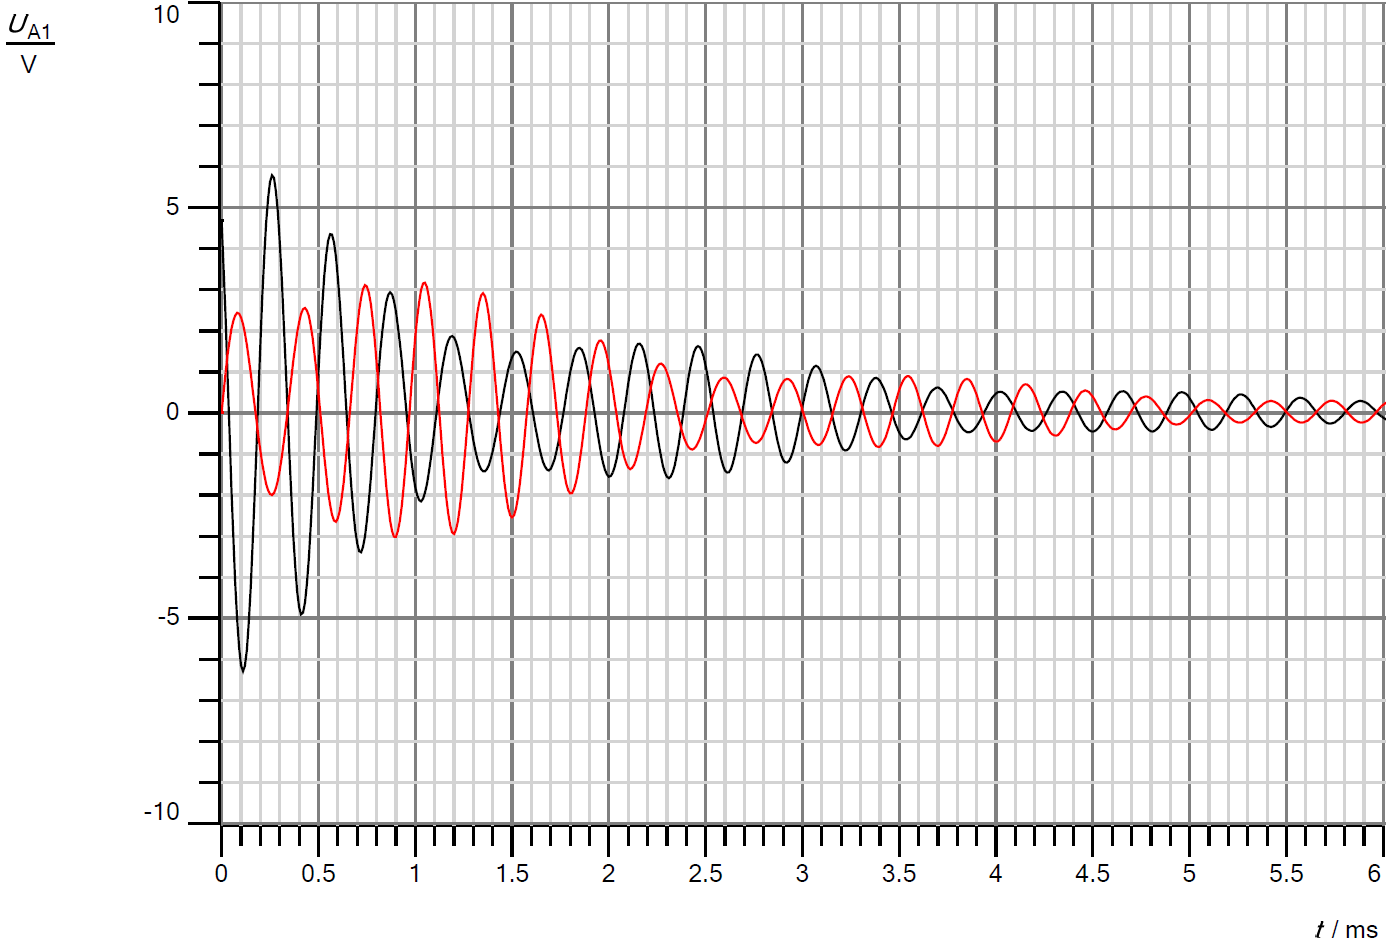
\includegraphics[width = .75\framewidth]{abbildungen/plotsLC/GegenGraph.PNG}
\caption{Zeitbereich der gegensinnigen Messung von Gruppe 1.}
\end{figure}
\end{frame}


\begin{frame}
\frametitle{Gleichsinnige - Zeitbereich}
\begin{figure}
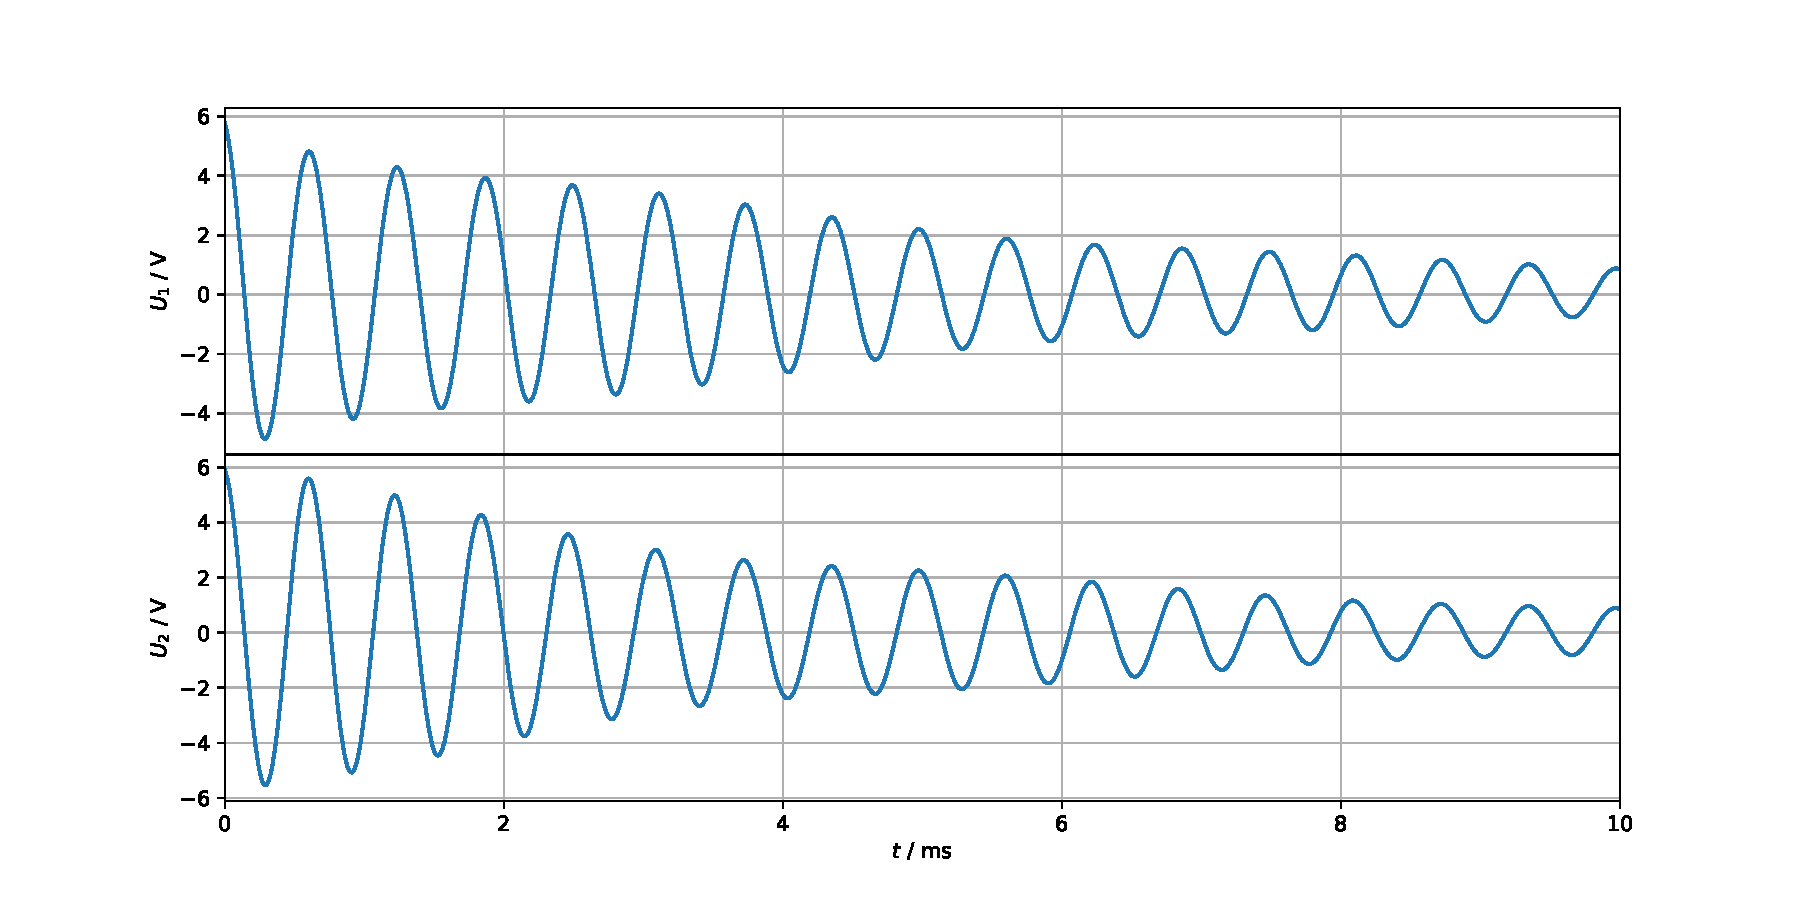
\includegraphics[width = \framewidth]{abbildungen/plotsLC/fundamental_roh.pdf}
\caption{Zeitbereich der gleichsinnigen Messung von Gruppe 2.}
\end{figure}
\end{frame}

\begin{frame}
\frametitle{Frequenzspektrum}
\begin{figure}
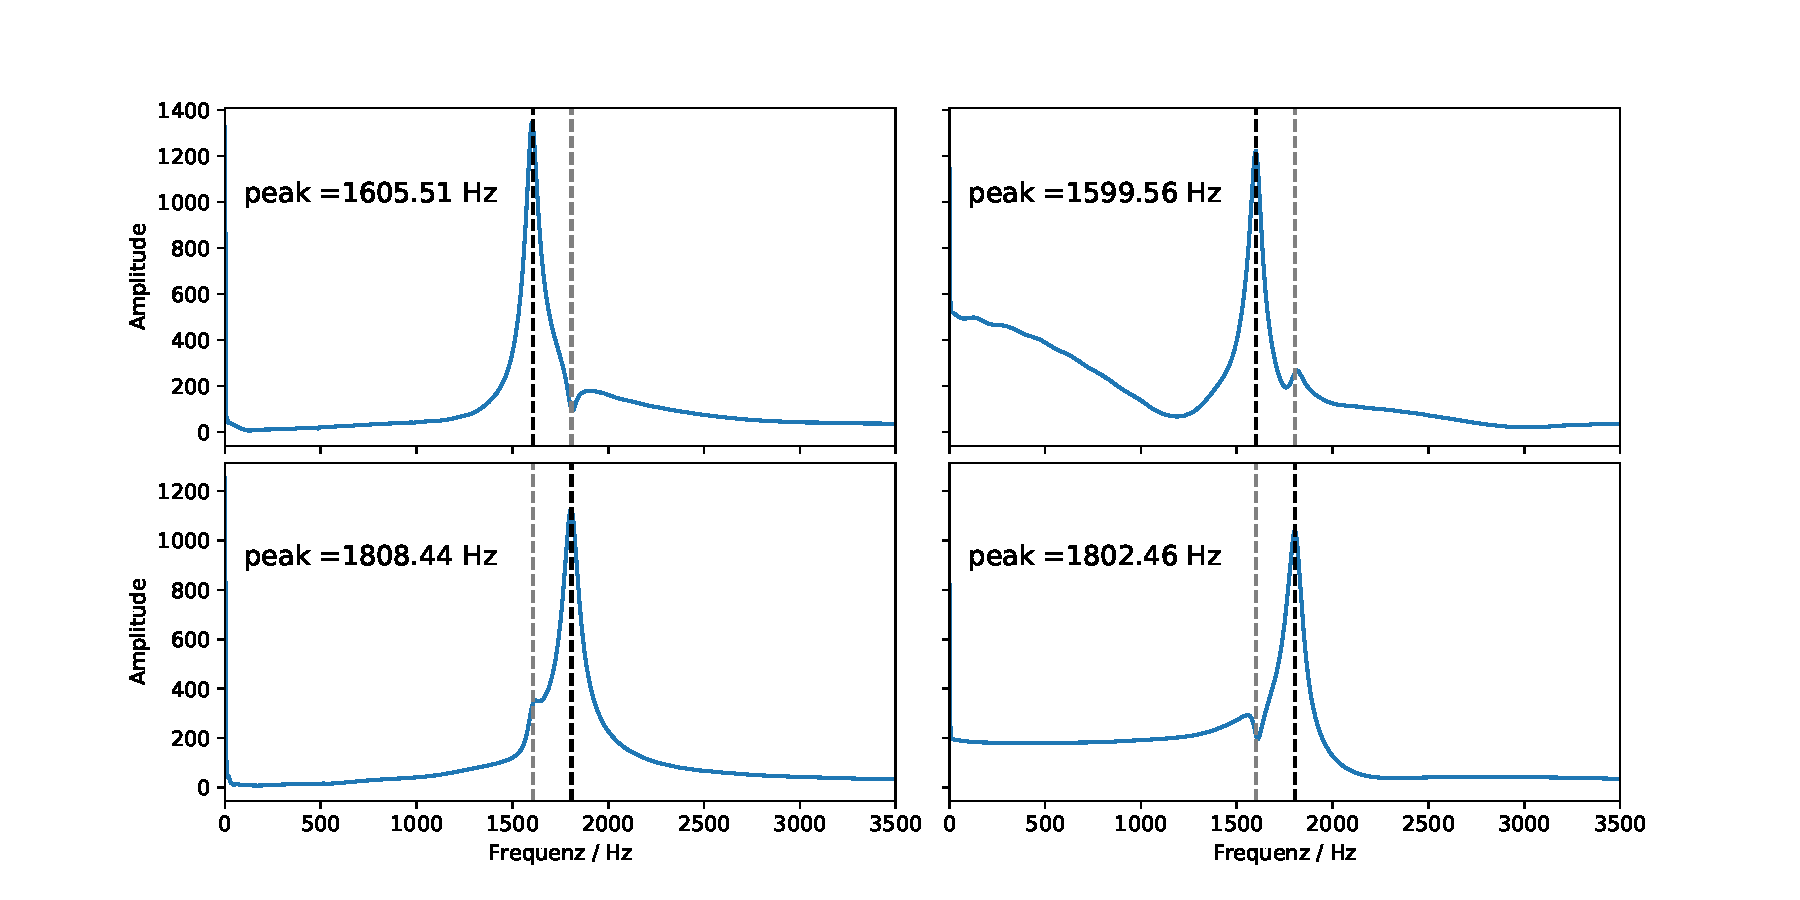
\includegraphics[width = \framewidth]{abbildungen/plotsLC/fundamental_fft.pdf}
\caption{Frequenzspektren der gleich- und gegensinnigen Messungen von Gruppe 2.}
\end{figure}
\end{frame}

\begin{frame}
\frametitle{Fazit}
\begin{itemize}
\item Messungen sehr schwer durchzuführen, da die Bauteile leicht verschieden sind und das Timing perfekt stimmen muss.
\item Erwartete, qualitative Effekte sind aufgetreten. Besonders gut im Frequenzspektrum erkennbar.
\end{itemize}
\end{frame}


\end{document}
